% Autor: Rami Boutassghount
% Website: https://ramiboutas.com/
% Linkedin: https://www.linkedin.com/in/ramiboutas/
% Twitter: https://twitter.com/ramiboutas
% Telegram: https://t.me/ramiboutas

\documentclass[tikz, convert={density=300}]{standalone}
\usepackage{tikz}
\usetikzlibrary{shapes.geometric, arrows}

\tikzstyle{startstop} = [rectangle, rounded corners, 
minimum width=3cm, 
minimum height=1cm,
text centered, 
draw=black, 
fill=red!30]

\tikzstyle{io} = [trapezium, 
trapezium stretches=true, % A later addition
trapezium left angle=70, 
trapezium right angle=110, 
minimum width=3cm, 
minimum height=1cm, text centered, 
draw=black, fill=blue!30]

\tikzstyle{process} = [rectangle, 
minimum width=3cm, 
minimum height=1cm, 
text centered, 
text width=3cm, 
draw=black, 
fill=orange!30]

\tikzstyle{decision} = [diamond, 
minimum width=3cm, 
minimum height=1cm, 
text centered, 
draw=black, 
fill=green!30]
\tikzstyle{arrow} = [thick,->,>=stealth]
\begin{document}

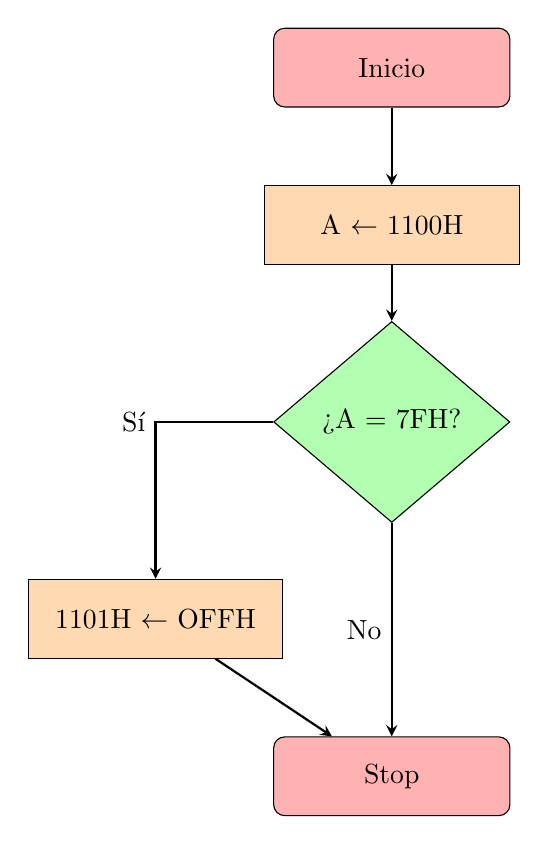
\begin{tikzpicture}[node distance=2cm]

\node (start) [startstop] {Inicio};
\node (pro1) [process, below of=start] {A $\leftarrow$ 1100H};
\node (dec1) [decision, below of=pro1, yshift=-0.5cm] { ¿A = 7FH? };
\node (pro2) [process, below of=dec1, yshift=-0.5cm, xshift=-3cm] {1101H $\leftarrow$ OFFH};
\node (stop) [startstop, below of=pro2, xshift=3cm] {Stop};

\draw [arrow] (start) -- (pro1);
\draw [arrow] (pro1) -- (dec1);
\draw [arrow] (dec1) -| node[anchor=east] {Sí} (pro2);
\draw [arrow] (dec1) -- node[anchor=east] {No} (stop);
\draw [arrow] (pro2) --++ (stop);


\end{tikzpicture}
\end{document}